\normalfalse \difficiletrue \tdifficilefalse
\correctionfalse

%\UPSTIidClasse{11} % 11 sup, 12 spé
%\newcommand{\UPSTIidClasse}{12}

\exer{Mouvement RR -- RSG  $\star\star$ \label{B2:13:PTSI:46}}
\setcounter{numques}{0}
\UPSTIcompetence{B2-13}
\index{Compétence B2-13-PTSI}
\index{Mécanisme à 2 rotations et RSG}
\index{Segway}
\ifcorrection
\else
\textbf{Pas de corrigé pour cet exercice.}
\fi

\ifprof
\else
Soit le mécanisme suivant.
\begin{center}
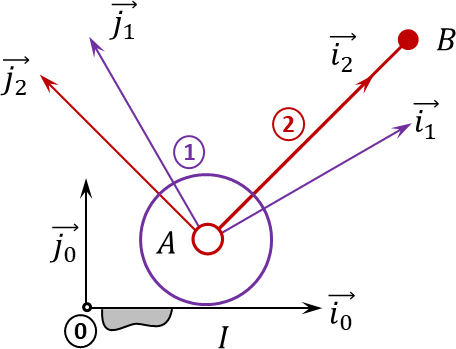
\includegraphics[width=\linewidth]{46_RR_RSG_01}
\end{center}
\fi


\question{Réaliser le paramétrage du mécanisme.}



\ifprof
\else

\footnotesize
\begin{center}
\begin{tabular}{|p{.9\linewidth}|}
\hline
Indications (à vérifier...) :
\begin{enumerate}
\item $\vectv{B}{2}{0} = L\varphip(t)\vj{2} +\thetap(t)\left(L\vj{1}-R\vi{0}\right) $.
\item  $\torseurcin{V}{2}{0} = \torseurl{\vecto{2}{0}=\left( \varphip(t)+\thetap(t) \right) \vk{0} }{ L\varphip(t)\vj{2} +\thetap(t)\left(L\vj{1}-R\vi{0}\right)}{B}$.
\item $\vectg{B}{2}{0} =  L\varphipp(t)\vj{2}-L\varphip(t)\left(\varphip(t)+\thetap(t) \right)\vi{2}  + \thetapp(t)\left(L\vj{1}-R\vi{0}\right) - L\thetap^2(t)\vi{1}$.
\end{enumerate} \\ \hline
\end{tabular}
\end{center}
\normalsize


\begin{flushright}
\footnotesize{Corrigé  voir \ref{B2:13:PTSI:46}.}
\end{flushright}%
\fi